%!TEX root = ./main.tex


\section{Background}

%Gaussian graphical models-------------------------------
\subsection{Gaussian Graphical Models}
\begin{frame}{Gaussian Graphical Models}
    Models for the \alert{conditional dependence structure} among variables, represented through an undirected graph $G=(V,E)$
    \begin{align*}
    \bm{y}_{1}, \ldots, \bm{y}_{n} \mid \bm{K} &\iid \mathcal{N}_{p}(\bm{0},\bm{K}^{-1})
    \end{align*}
Conditional independence described through a \alert{map} between a \alert{graph} and a family of multivariate \alert{probability models}
\begin{align*}
Y_{i}\indep Y_{j} \mid Y_{-(ij)} \iff (i,j) \notin E \iff k_{ij}=0
\end{align*}
Usual prior for $\bm{K}$ conditionally to the graph is a G-Wishart
\begin{align*}
    \bm{K} \mid G &\iid \GWish(b,D)
\end{align*}
$G$ is a r.v. in the space of undirected graphs with $p$ nodes.\\
If we assume a possible \alert{grouping} of the variables, we need a prior $\pi(G)$ that induces a \alert{block structure on its adjacency matrix}.
\end{frame}


%%TO DO @Teo 
%Add bold sigma
%Add the image - STAVO PENSANDO, MA SE NE METTESSIMO DUE? UNA CON UN GRAFO CON ELEMENTI DA 1 A P STRUTTURA E UNA TABELLA - OK CHE E' SIMILE A QUELLO DI COLOMBI BUT STILL
%%

 

%Stochastic Block Models -----------------------
\subsection{Stochastic Block Models}
\begin{frame}{Stochastic Block Models for the prior on $G$}

Given a random network, SBM \alert{infer a node partition} based on similarity of connectivity patterns. Let
\begin{itemize}
    \item $H$ be the fixed number of clusters
    \item $\bm{z} \in \mathbb{R}^p$ be the vector of group memberships, $z_{i} \in \{1,\ldots,H\}$
\end{itemize} 
Then the model of the graph conditionally on $\bm{z}$ is the following
\begin{align*}
    P((i,j)\in E\mid \bm{z},Q) &= Q_{z_{i} z_{j}},\,\text{independent}\\
    Q_{rs} &\ind \Beta(a,b),\quad 1\leq r\leq s\leq H\\
    \bm{z} &\sim f_{z}(\bm{z})
\end{align*}
Problems:
\begin{itemize}
    \pause
    \item {\small How to \alert{identify the number of clusters $H$}?}
    \pause
    \item {\small How to model \alert{constraints on the ordering of the nodes} when generating the partition?}
\end{itemize}

% \begin{center}
%     Critical task: \alert{identification of the number of clusters $H$}
% \end{center}

\end{frame}
















%Changepoint models------------------
\subsection{Changepoint Models}
\begin{frame}{Changepoint Models}
    %\fg{0.4}{changepoint}
    Let $\bm{y}=(y_{1},\ldots,y_{n})$ be \alert{ordered} observations, each depending on a parameter $\vartheta_{i}$.
    Consider a process where the underlying generating mechanism changes at time $\tau_{j}$, $j=1,\ldots,k+1$, where $\tau_{j},k$ are unknown. The likelihood can be modeled as
    \begin{align*}
        f(y_{1},\ldots,y_{n} \mid \vartheta_1, \vartheta_2, \ldots, \vartheta_{k+1}, \bm{z})=\prod_{j=1}^{k+1} \prod_{i=\tau_{j-1}+1}^{\tau_j} f(y_i \mid \vartheta_j),
        \qquad
        k=\sum_{i=1}^{n-1} z_i
    \end{align*}
    where $\tau_j$ are called \alert{changepoints} and $z_{i} = 1$ if $i$ is a changepoint, $0$ otherwise.
    We are interested in \alert{generating a random partition with ordering constraints}
    \begin{align*}
        \pi(\bm{z}, \bm{\vartheta} \mid \bm{y}) & \propto f(\bm{y} \mid \bm{\vartheta}, \bm{z}) \pi(\bm{\vartheta} \mid \bm{z}) \pi(\bm{z})
    \end{align*}
    % We will choose as prior $\pi (\bm{z})$ the one proposed by Martinez et. al (2014)
    % \begin{equation*}
    %     \mathbb{P}\left(\rho_n=\left(n_1, \ldots, n_k\right)\right)=\frac{n !}{k !} \frac{\prod_{i=1}^{k-1}(\theta+i \sigma)}{(\theta+1)_{n-1 \uparrow}} \prod_{j=1}^k \frac{(1-\sigma)_{n_j-1 \uparrow}}{n_{j} !}
    % \end{equation*}
\end{frame}


\begin{frame}
To define the distribution of $\bm{z}$ we assign a probability law over the space of all \alert{admissible} partitions.

\pause

Let $\rho_p=\left\{C_1, \ldots, C_M\right\}$ be a partition of the $p$ nodes.
\[
    \rho_p \text{ is admissible} \iff \forall x \in C_i, y \in C_{j}, \; i<j \text{ implies } x < y
\]
% In other words, if groups are contiguous.
%Martínez and Mena (2014) assign
\cite{martinezNonparametricChangePoint2014} assign
\begin{equation*}
    P\left(\rho_p=\left\{C_1, \ldots, C_M\right\}\right)
    =
    p'(n_1, \ldots, n_k)=
    \begin{cases}
        \binom{n}{n_1, \ldots, n_k} \frac{1}{k !} p(n_1, \ldots, n_k), & \rho_p \text{ admissible}\\
        0, & \rho_p \text{ not admissible}
    \end{cases}
\end{equation*}
where $n_j=\left|C_j\right|$, $p(n_1, \ldots, n_k)$ any Exchangeable Partition Probability Function (EPPF).

The vector $\bm{z}$ is derived by setting
\[
z_i=m \iff i \in C_m, \quad i=1, \ldots, p, \quad m=1, \ldots, M.
\]
\end{frame}







%----------------------------------------
% Project goals
%-------------------------------------
\section{Project goals and next steps}
\begin{frame}{Goal of the project and next steps}

\vspace*{0.5cm}
\begin{columns}

    \begin{column}{0.4\textwidth}
        \alert{Goal:} propose a \alert{new prior} that accounts for
        %a random partition of the nodes, respects their ordering constraints and allows to learn a block structured graph
        \begin{itemize}
            \item Ordering Constraint: taking advantage of the study of changepoint models
            %\item Random partition: using nonparametric prior on ordered partitions
            \item Block Structure: using a stochastic block model prior
        \end{itemize}
    \end{column}
    \begin{column}{0.6\textwidth}
        \begin{align*}
        \bm{y}_1, \ldots, \bm{y}_n \mid \bm{K} & \iid \mathcal{N}_p(\mathbf{0}, \bm{K}^{-1} ) \\
        \bm{K} \mid G & \sim \GWish(b, D)\\
        P((i,j)&\in E\mid \bm{z},Q) = Q_{z_{i} z_{j}},\,\text{independent}\\
            Q_{rs} \mid \bm{z} &\ind \Beta(a,b), 1\leq r\leq s\leq H\\
        \rho_p & \sim \mathcal{L}\left(\rho_p\right)
        \end{align*}  
    \end{column}
\end{columns}
\vspace*{0.5cm}


\alert{Next steps:}
\begin{itemize}
\item understand the nonparametric prior on ordered partitions
\item implement the sampling strategy
\end{itemize}

\end{frame}

\begin{frame}{Main references}
    % GGM
    \nocite{colombiLearningBlockStructured2022a}
    \nocite{mohammadiBayesianStructureLearning2015a}
    % SBM
    \nocite{legramantiExtendedStochasticBlock2022}
    % Changepoint
    \nocite{bensonAdaptiveMCMCMultiple2018}
    \nocite{martinezNonparametricChangePoint2014}
    
    
    %biblatex
    \printbibliography
    \renewcommand*{\bibfont}{\small}
    %bibtex
    %\bibliographystyle{plain} % We choose the "plain" reference style
    %\bibliography{bibliography} % Entries are in the refs.bib file
\end{frame}

\begin{frame}[plain]
    % Add background to content page
    \AddToShipoutPictureFG*{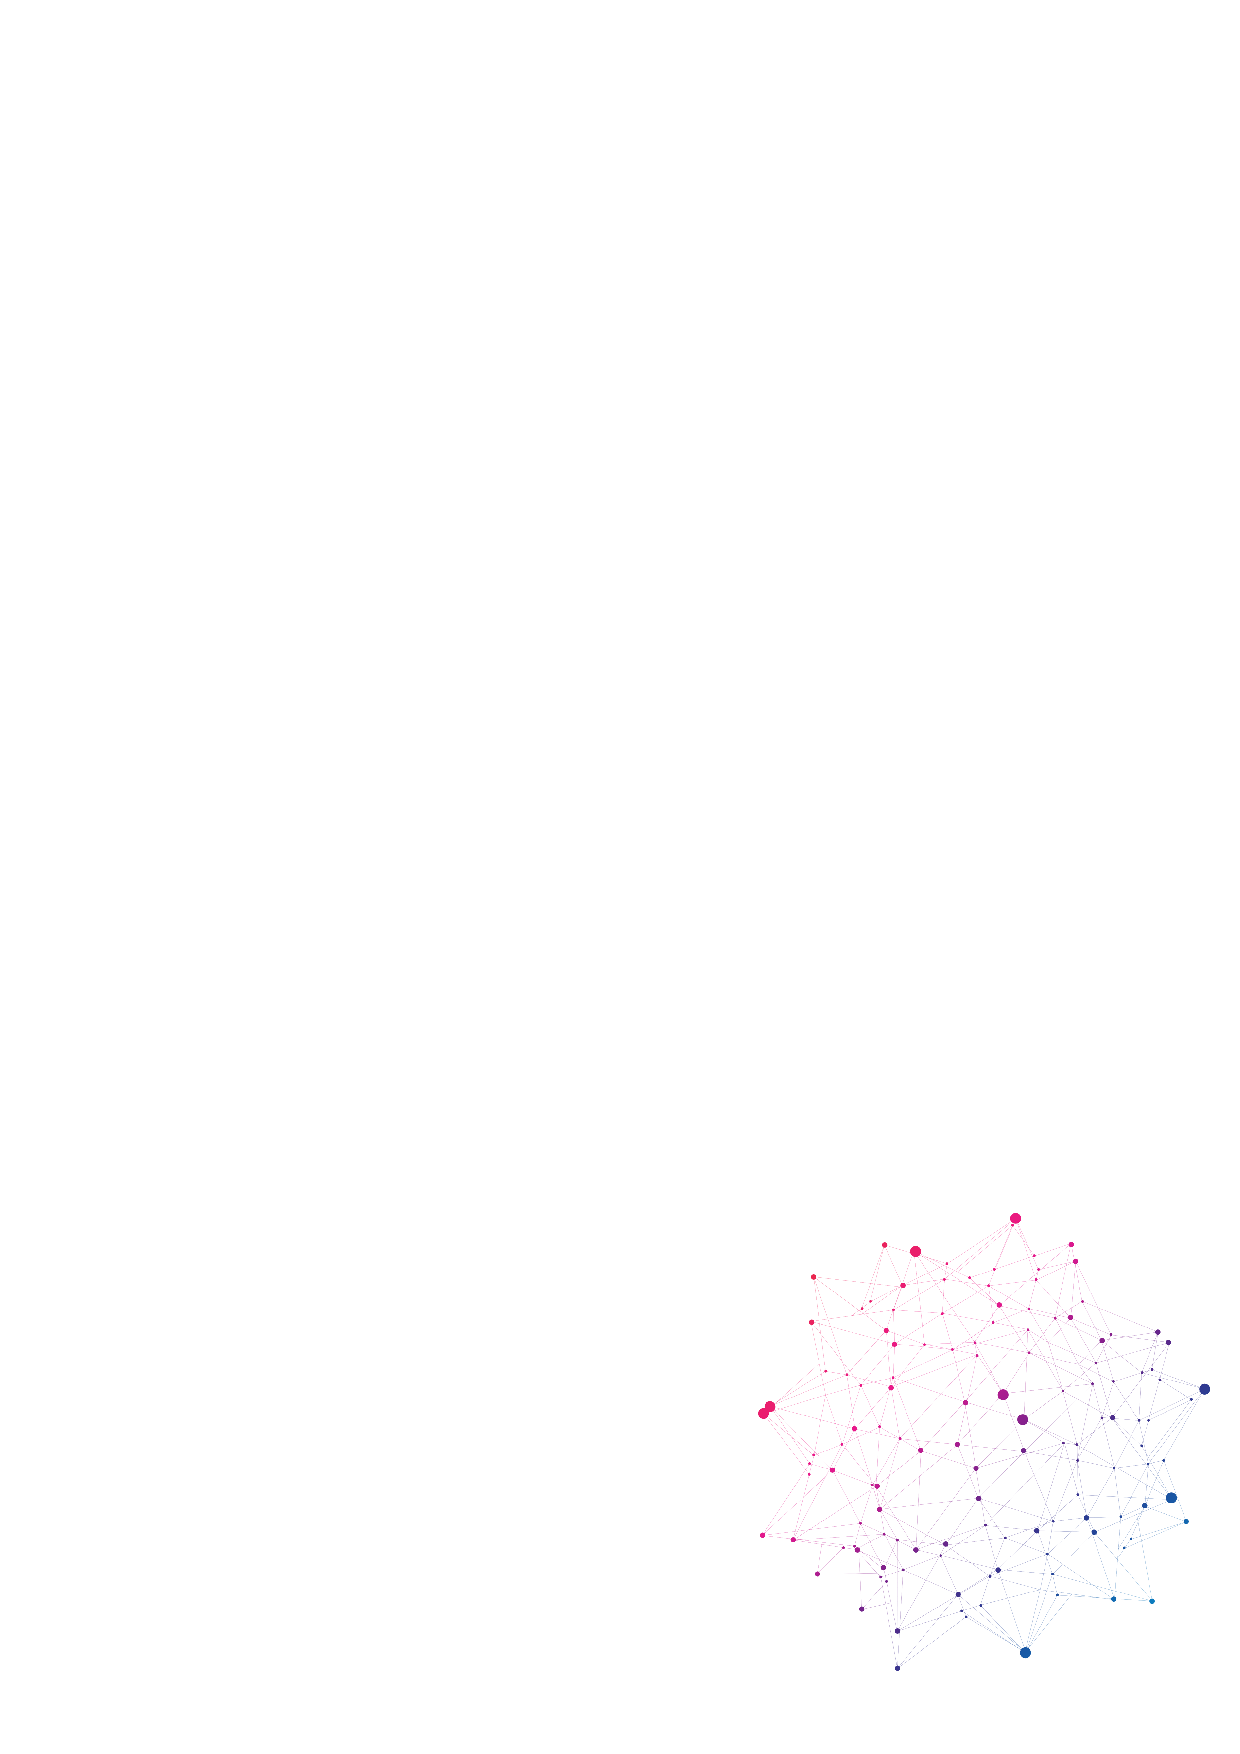
\includegraphics[width=\paperwidth]{Images/background.pdf}}
    \vspace*{1.2cm}
    \hspace*{1cm}{\Large Thank you!}\\
    \vspace*{0.6cm}
    \pause
    \hspace*{1cm}{\Huge \alert{Any questions?}}
\end{frame}


















%tenere?
\section*{Extra}
%Stochastic Block Models -----------------------
\begin{frame}{Stochastic Block Models for the prior on G}

\begin{align*}
    G_{ij} \mid \Theta,\bm{z} &\iid \Be(\theta_{ij}),  G \in \mathbb{R}^{p \times p}, \quad \theta_{ij} = \Theta_{z_{i}z_{j}}, \quad 1 \le i < j \le p \\ 
    \Theta_{z_{i}z_{j}} &\iid \Beta(\alpha, \beta)\\
    \bm{z} &\iid \pi_{z}(\bm{z}), \quad \bm{z} \in \mathbb{R}^p
\end{align*}
$\Theta$ can be marginalized out via beta-binomial conjugacy.
%Tattica: farei comparire la figura con un tap, e intanto si commenta che "per brevità non entriamo nel dettaglio ma se sono interessati si"
\fg{0.9}{sbm}
%Aggiungere da dove viene la caption
 %% Critical task: \alert{identification of the number of clusters H}
{\scriptsize From \cite{colombiLearningBlockStructured2022a}}
\end{frame}














\begin{frame}{Choosing the number of clusters $H$}

$H$ is usually chosen using data driven methods \alert{before} estimating the model. However
\begin{itemize}
    \item uncertainty quantification for $H$ at this stage is ignored
    \item the model does not account for new clusters (\alert{prediction})
\end{itemize}
\pause
Among others, \cite{legramantiExtendedStochasticBlock2022} proposed the \alert{Extended Stochastic Block Models (ESBM)}, which use priors for $\bm{z}$ that naturally allow to adaptively modify the number of groups $H$, \emph{e.g.},
\begin{itemize}
    \item Finite Dirichlet
    \item Infinite Dirichlet
    \item Finite mixtures with a random number of components
\end{itemize}

\pause
\begin{center}
    \alert{None of the ESBM models pose constraints\\
    on the ordering of the nodes when generating the partition,\\
    that may be of relevance in real-life context (i.e., gene expression).}    
\end{center}


\end{frame}